\chapter{Problem Formulation and State Of The Art}

\section{Definition}

In order to estimate the percentage of tumoural cells we decided to solve other problem. Instead of just predicting a number from a WSI, which would make the problem a logistic regression problem, we decided to segment and classify every cell to later count them and compute the percentage. The latter seems to be a more complex and difficult problem but it is not. Let's describe mathematically each problem in order to analyse each of them and come to the conclusion that the former is a quite unfeasible problem given our resources.

First, let's denote by $\mathcal{X}$ and $\mathcal{Y}$ the input and output space of the problem. We expect to find a function $f : \mathcal{X} \to \mathcal{Y}$ that effectively predicts the correct percentage given the WSI. Any WSI is no more than a collection of pixels, for that reason they can be viewed as very high dimensional vectors $\mathcal{X} = \mathbb{R}^N$, with $N > 10^{9}$ \cite{DICOM}. Similarly, the percentage is just a number between 0 and 1, so $\mathcal{Y} = [0,1]$.

Now, the logistic regression approach consists of finding such function from a family of parametric models $\mathcal{F}_\theta = \{ f_\theta | f_\theta : \mathcal{X} \to \mathcal{Y} \}$ while the segmentation approach tries to find $f$ differently. It first divides the WSI into patches. Then, each patch is processed independently to obtain pixel-wise predictions which are then used to compute the percentage. So, the family of parametric models now in consideration is $\mathcal{G}_\theta = \{ g_\theta | g_\theta : \mathcal{X}_s \to \mathcal{X}_s,\ \mathcal{X}_s \subset \mathcal{X} \}$ where $\mathcal{X}_s$ represents the space of images of 1024 by 1024 pixels, meaning $\text{dim}(\mathcal{X}_s) \approx 3.1 \cdot 10^6$. Given any segmentation model $g_\theta$ we construct its regression counterpart $f_\theta$ as described in the following commutative diagram. 

\[ \begin{tikzcd}
\mathcal{X} \arrow{r}{f_\theta} \arrow[swap]{d}{s} & \mathcal{Y} \\%
\mathcal{X}_s^P \arrow{r}{\tilde{g}_\theta}& \mathcal{X}_s^P \arrow{u}{c}
\end{tikzcd}
\]

Where we have extended $g_\theta$ to several patches by applying it independently to all of them.

\begin{align}
\begin{split}
\tilde{g}_\theta : \mathcal{X}_s^P& \to \mathcal{X}_s^P\\
(x_1, ..., x_P)& \mapsto (g_\theta(x_1), ..., g_\theta(x_P))
\end{split}
\end{align}

And the $s$ and $c$ functions refer to the split and count operations. Given a WSI it is split into several patches, for each patch, every cell is segmented and then all the tumoural and healthy cells are counted.

Without making any further assumptions about the families of functions we can derive some important insights about the advantages and disadvantages of each approach. First of all, it is clear that in the first approach the models have access to a wider context. Considering independent patches limits the ability to take into account global information. The presence of cilium in the middle of a WSI cannot be taken into account when classifying the border of the tissue. But this disadvantage is not such a big deal. In reality, two far away lymphocytes are not really interacting with each other. And erythrocytes only affect immediate cells. So, a 1024 by 1024 window does not seem to be a big problem. On the other hand, if we look at the dimensionality of input and output spaces we see a clear difference between the two approaches. For $\mathcal{F}_\theta$ the input space has a huge dimensionality while the output is uni-dimensional. In contrast, for $\mathcal{G}_\theta$ the input and output space both have the same dimensionality which is several orders of magnitude smaller than the dimensionality of $\mathcal{X}$. This makes the first approach quite prone to the curse of dimensionality \cite{AnalyticsVidhya}. Even worse, we have just one number per each WSI. Even a simple regression problem needs more than 30 samples to have a reasonable amount of uncertainty. When we had to choose the approach in september 2022 there were only 10 available WSI which made the decision obvious.

\section{Data labelling}\label{sec:data}

As stated in the previous section we have access to few WSI but each WSI contains a lot of information. One can extract hundreds of patches from surgical biopsies made by thoracotomy, and even in needle biopsies it is possible to obtain more than ten patches. However, those images are of no use without their corresponding labels. To illustrate what we are referring to, look at \autoref{fig:labels} below.

\begin{figure}[ht]
  \centering
  \begin{subfigure}[b]{0.45\textwidth}
    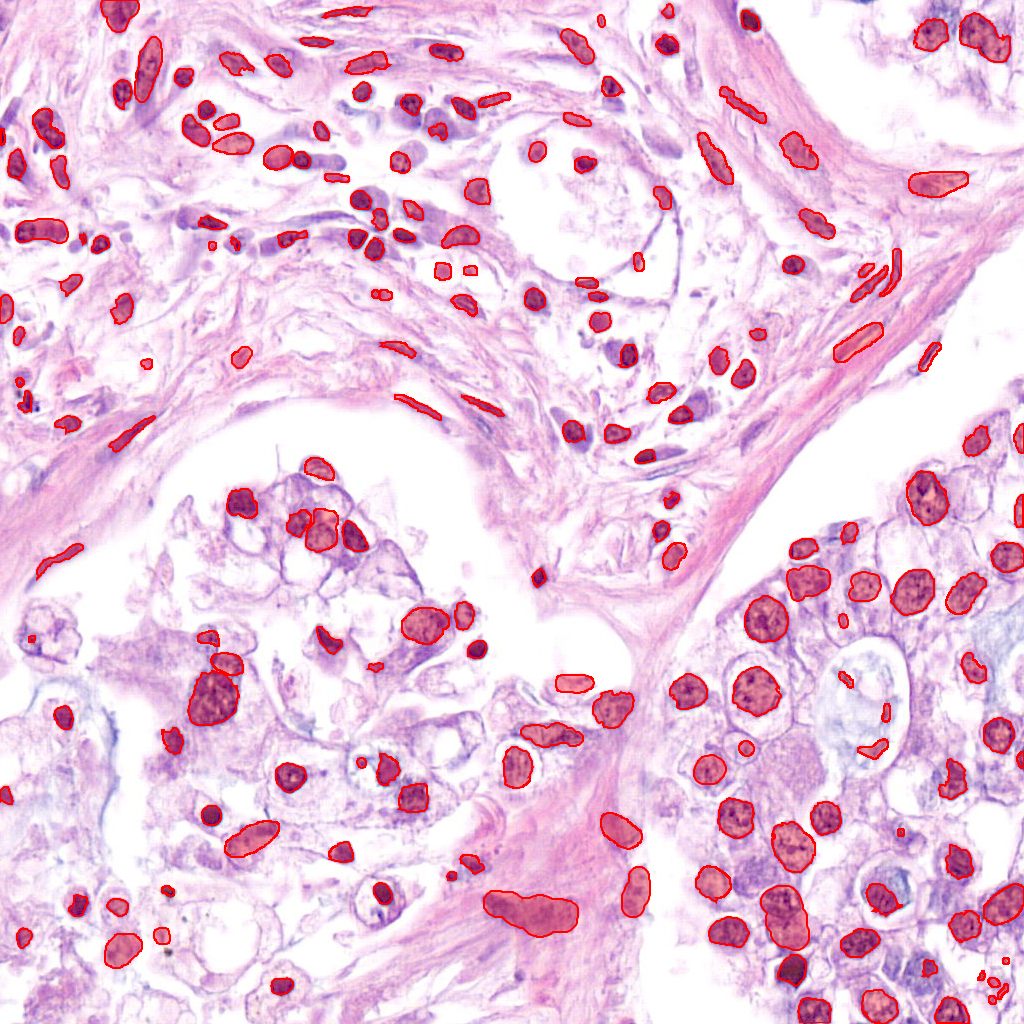
\includegraphics[width=\textwidth]{imgs/seg.png}
    \caption{Segmentation}
    \label{fig:seg}
  \end{subfigure}
  \hfill
  \begin{subfigure}[b]{0.45\textwidth}
    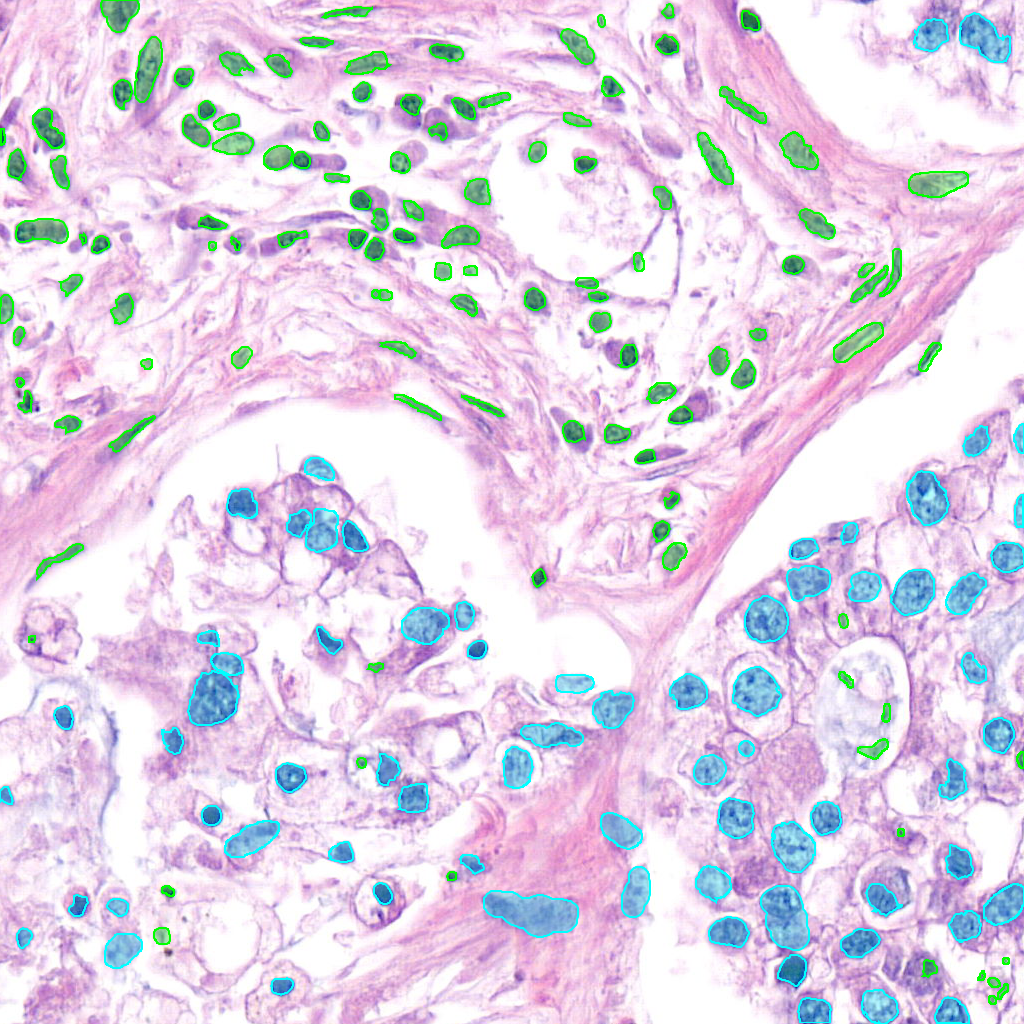
\includegraphics[width=\textwidth]{imgs/overlay.png}
    \caption{Classification}
    \label{fig:class}
  \end{subfigure}
  \caption{Visualisation of the kind of labels that are needed. For each cell it is required to have its contour, as seen in the left, together with their corresponding class as seen in the right. Blue means tumoural and green non-tumoural.}
  \label{fig:labels}
\end{figure}

The ground truth (GT) used to train the models needs to be handcrafted, which is a tedious process. To alleviate the amount of work required, an iterative procedure was designed. In a first step made by David Anglada and Feliu Formosa, the max-tree \cite{maxtree} was used to create rough segmentations of 24 patches that were later reviewed and improved by the students. Those initial labels were used to train Hovernet \cite{hovernet}, explained in detail in \autoref{sec:vision}. Using that newly trained model, 20 more images were annotated and reviewed by me. Then, Hovernet was trained again using those 44 images and used to infer the GT of 41 more patches. Only after carefully correcting all the 85 slices, would the pathologist Irene Sansano Valero start reviewing the dataset. The whole process took around 100 hours of human labour, around 20 hours of GPU computation and 10 hours of expert human labour.

\section{Computer vision algorithms}\label{sec:vision}

In this section I will provide a brief survey about the state of the art in segmentations problems and a detailed explanation of Hovernet \cite{hovernet} which is the model used in the first phase of our method.

The first deep learning attempt at biomedical segmentation was made by Olaf Ronneberger et al. \cite{unet}. They proposed an encoder-decoder architecture as shown in \autoref{fig:unet}.

\begin{figure}[ht]
    \centering
    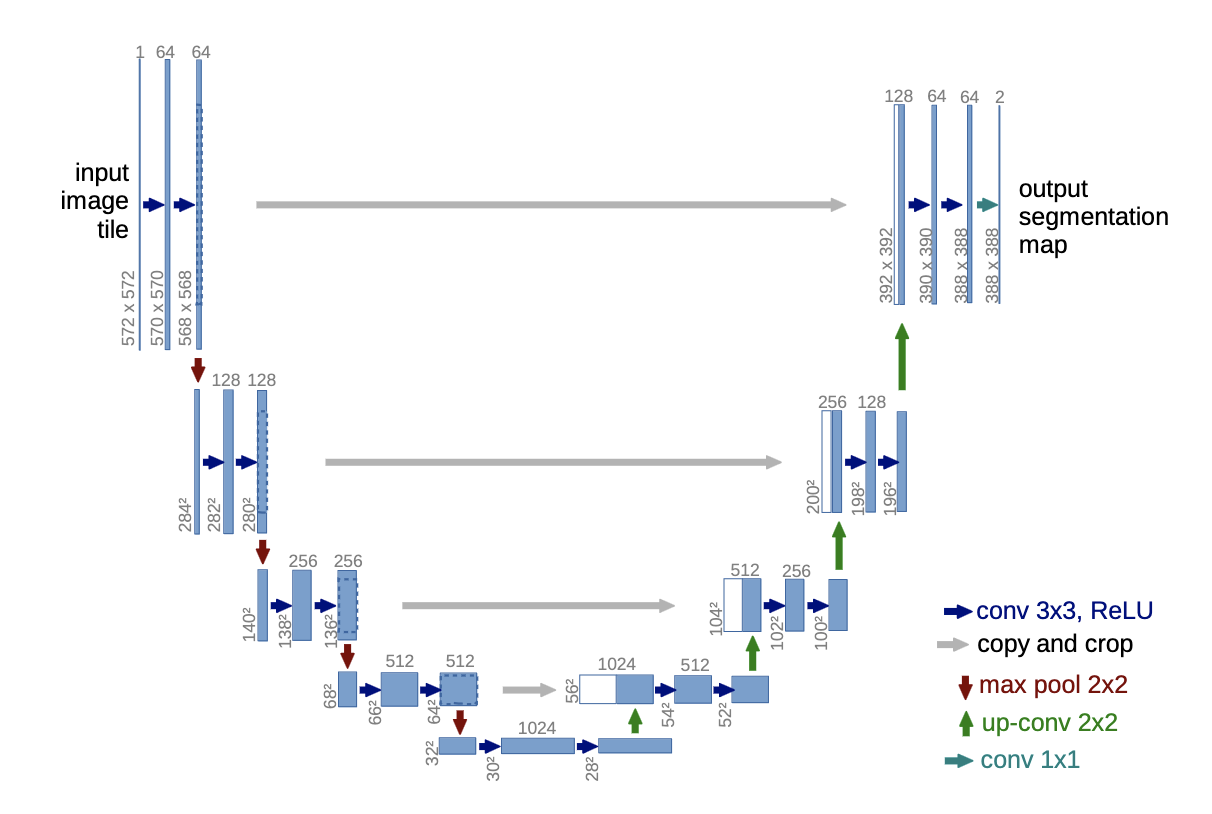
\includegraphics[width=\textwidth]{imgs/unet.png}
    \caption{Original U-net architecture. It was composed by convolutional layers, pooling layers and residual connections.}
    \label{fig:unet}
\end{figure}

That architecture was improved recently with the development of transformers \cite{transformer}. In 2021 Jieneng Chen et al. invented TransUNet \cite{transunet} and later on in 2022 Jeya Maria Jose Valanarasu et al. created UNeXt \cite{unext}. I will not dive into the specifics of those architectures but rather comment on their limitations and why we couldn't use them. The key limitation is their sample efficiency. Even though transformers are more sample efficient in reinforcement learning than previous deep learning methods \cite{micheli2023transformers}, they still require a fair amount of data. In Jeya Maria Jose Valanarasu et al. \cite{unext} they used two datasets of 2594 and 647 images respectively. That is at least an order of magnitude more than what we could obtain. The other option, TransUNet \cite{transunet}, was tried in a dataset with 3779 computer tomography (CT) images, yet too much for us. Apart from that, the problem they tackled was organ segmentation, which is quite different from cell segmentation. In order to achieve better sample efficiency, a method with specific inductive biases is needed.

As explained in \autoref{sec:data}, the max-tree \cite{maxtree} can give good results at detecting cell contours while using no data at all. The algorithm used morphological properties of the cells to distinguish them from the background. That set a precedent, morphological algorithms could help us reduce the amount of data needed. Another important morphological algorithm is the watershed \cite{watershed}. It is known for creating accurate contours if the energy landscape is properly defined. Hovernet \cite{hovernet} combines both the U-net architecture with the watershed algorithm to produce cell segmentations and classify them. An overview is on \autoref{fig:hovpipe}.

\begin{figure}[ht]
    \centering
    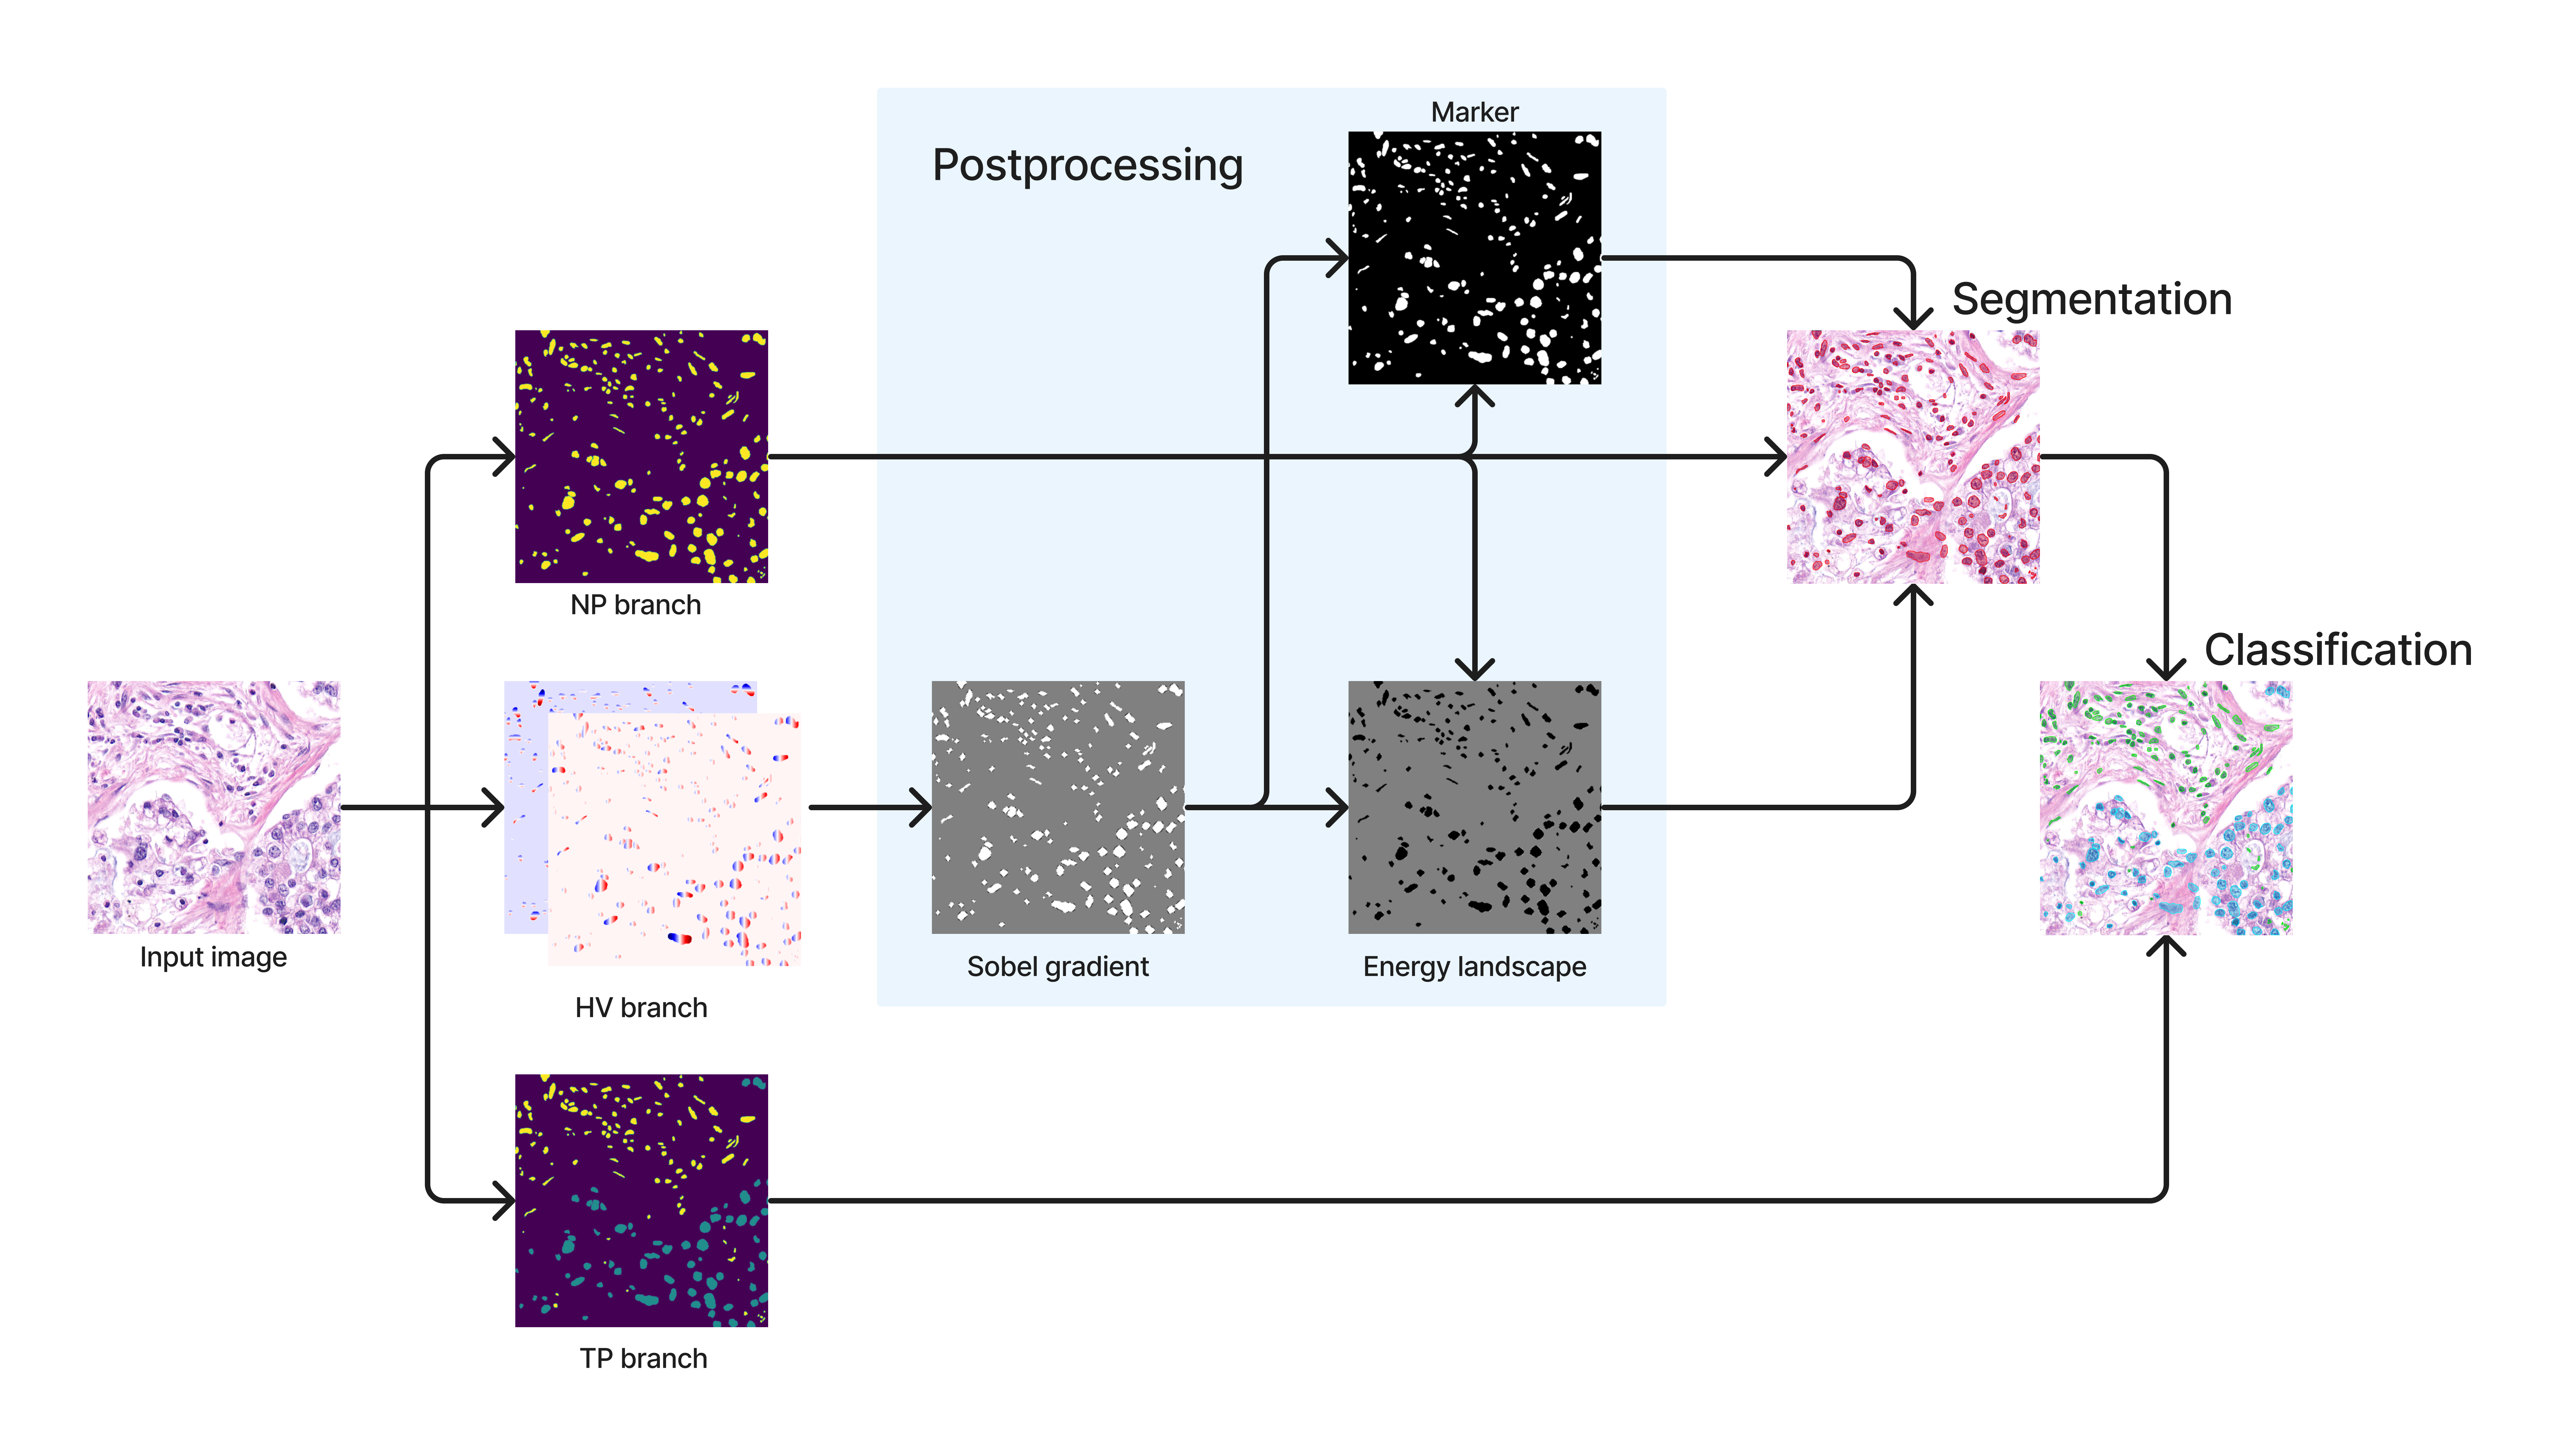
\includegraphics[width=\textwidth]{imgs/hovpipe.png}
    \caption{Overview of the Hovernet method. It has three branches that predict different maps derived from the GT. In a post-processing step all the maps are combined using the watershed algorithm with carefully designed energy landscapes and markers.}
    \label{fig:hovpipe}
\end{figure}

Hovernet employs the same encoder-decoder architecture as U-net but it combines three different decoders with only one shared encoder. Each of the three decoders is trained to infer a different property from the GT. The NP branch separates the cells from the background, ignoring their class. The HV branch predicts horizontal and vertical distances from each pixel to the nuclei of the nearest cell. And the TP branch predicts the GT as is. Everything is trained end-to-end under one single loss function, which is shown below

\begin{align}
    \mathcal{L} &= \lambda_{mse}^{HV}\mathcal{L}_{mse}^{HV} + \lambda_{msge}^{HV}\mathcal{L}_{msge}^{HV} + \lambda_{bce}^{NP}\mathcal{L}_{bce}^{NP} + \lambda_{dice}^{NP}\mathcal{L}_{dice}^{NP} + \lambda_{bce}^{TP}\mathcal{L}_{bce}^{TP} + \lambda_{dice}^{TP}\mathcal{L}_{dice}^{TP} \\
    &= \frac{\lambda_{mse}^{HV}}{B}\left( \sum_{i=0}^{B} \| H(x_i) - h_i \|_2^2 + \sum_{i=0}^{B} \| V(x_i) - v_i \|_2^2 \right) \\
    &+ \frac{\lambda_{msge}^{HV}}{B}\left( \sum_{i=0}^{B} \| \nabla H(x_i) - gh_i \|_2^2 + \sum_{i=0}^{B} \| \nabla V(x_i) - gv_i \|_2^2 \right) \\
    &+ \frac{\lambda_{bce}^{NP}}{B} \sum_{i=0}^B \sum_{j=0}^{D} (y_{i}^{NP})_j \log (NP(x_i)_j) \\
    &+ \frac{\lambda_{dice}^{NP}}{B} \sum_{i=0}^B \left(1 - \frac{\sum_{j=0}^D NP(x_i)_j (y_{i}^{NP})_j}{\sum_{j=0}^D (NP(x_i)_j)^2 + \sum_{j=0}^D ((y_{i}^{NP})_j)^2}\right)\\
    &+ \frac{\lambda_{bce}^{TP}}{B} \sum_{i=0}^B \sum_{j=0}^{D} (y_{i}^{TP})_j \log (TP(x_i)_j) \\
    &+ \frac{\lambda_{dice}^{TP}}{B} \sum_{i=0}^B \left(1 - \frac{\sum_{j=0}^D TP(x_i)_j (y_{i}^{TP})_j}{\sum_{j=0}^D (TP(x_i)_j)^2 + \sum_{j=0}^D ((y_{i}^{TP})_j)^2}\right)
\end{align}

\noindent where all the $\lambda$ are hyperparameters, the letter $y$ denotes GT in any form, $h$ and $v$ are horizontal and vertical GT maps, $gh$ and $gv$ are the gradients of horizontal and vertical maps, $D$ is the number of pixels in any image, $B$ is the batch size, $\| \cdot \|_2^2$ is the $L_2$ norm, $H(\cdot)$ and $V(\cdot)$ are the outputs of the HV branch, $NP(\cdot)$ the output of the NP branch and $TP(\cdot)$ the output of the TP branch.

After the model is trained, it can be used for inference in addition with a post-processing phase which consists of the watershed algorithm. This particular watershed requires an energy landscape which defines the space where the flooding is made and a marker that contains the starting points to start the flooding. Both are defined below

\begin{align}
    E &= (1 - \mathcal{S}_m(\bX)) \odot NP(\bX) \\
    M &= \text{ReLU}(NP(\bX) - \mathcal{S}_m(\bX))
\end{align}

\noindent being $E$ the energy and $M$ the marker. In those equations $\bX$ refers to the input image, ReLU is the rectified linear unit \cite{relu}, $\odot$ is the element-wise multiplication, also referred to as Hadamard product, and $\mathcal{S}_m(\bX)$ is the thresholded gradient of the HV branch as expressed here

\begin{equation}
    \mathcal{S}_m(\bX) = \max(S_x * H(\bX), S_y * V(\bX))
\end{equation}

\noindent where $S_x$ and $S_y$ are Sobel filters \cite{sobel} and $*$ is the convolution operation. The whole process can be visualized in \autoref{fig:hovpipe}. 

%% Postprocessing step

\section{Graph neural networks}\label{sec:gnn}

Having described the state of the art for computer vision, let's introduce the state of the art of graph neural networks as well. There are more than 50 different possible architectures \cite{graph_survey} and more than 300.000 possible configurations \cite{you2021design}. However I will focus mainly on two of the most popular architectures: graph convolution and graph attention. Both can be used for node classification which is what we are interested about since we are going to treat cells as nodes. More on that description in \autoref{sec:descr}.

\subsection{Graph convolution}\label{sec:gcn}

This architecture was proposed by Thomas N. Kipf et al. \cite{graphconv} in 2016 and has been cited almost ten thousands times as of this date. The main idea is to adapt the notion of convolution from images to graphs. An illustration of the concept can be seen in \autoref{fig:conv_comp}.

\begin{figure}[ht]
    \centering
    \begin{subfigure}[b]{0.4\textwidth}
        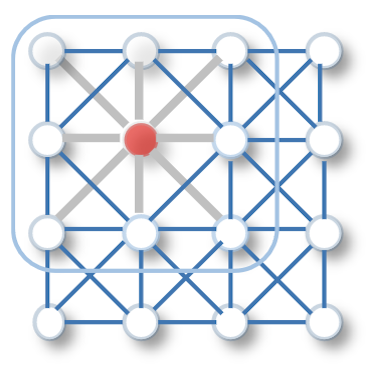
\includegraphics[width=\textwidth]{imgs/conv.png}
        \caption{2D Convolution where each pixel can be considered a node connected to all its adjacent pixels. This operation returns the weighted average of adjacent pixels for each node.}
    \end{subfigure}
    \hfill
    \begin{subfigure}[b]{0.4\textwidth}
        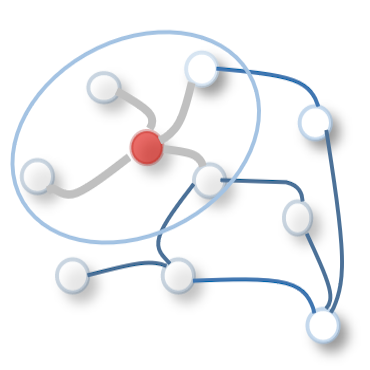
\includegraphics[width=\textwidth]{imgs/graph conv.png}
        \caption{Graph Convolution where the weighted average is taken with respect to adjacent nodes. There is no notion of pixels and each node has no absolute spatial coordinates.}
    \end{subfigure}
    \caption{Visualisation of 2D Convolution vs Graph Convolution taken from \cite{graph_survey}.}
    \label{fig:conv_comp}
\end{figure}

Mathematically, the graph convolution operation as expressed in \cite{graphconv} can be defined as shown below

\begin{equation}
    \bh_j^{(l+1)} = \sigma \left(\bb^{(l)} + \sum_{k \in \mathcal{N}_j} \frac{1}{c_{jk}} \bW^{(l)}\bh_k^{(l)}\right)
\end{equation}

\noindent where $\bb^{(l)}\in \R^d, \bW^{(l)} \in \R^{d\times d}$ are the bias and weights of the layer, $\mathcal{N}_j$ is the set of neighbours of node $j$, $c_{jk} = \sqrt{|\mathcal{N}_j|\cdot |\mathcal{N}_k|}$ is a normalisation factor and $\sigma$ is an activation function. The vectors $\bh_k^{(l)}$ are the hidden embeddings of the network for each layer, being $\bh_k^{(0)}$ an initial vector containing any relevant information about the node. That information can be the area of the cell, the average colour, or even a prior distribution for the class label. In the last layer, the weight matrix is of dimensions $C \times d$, where $C$ is the number of classes or $1$ if $C=2$ and the activation function is either the sigmoid for a binary problem or the softmax \cite{softmax} for a multi-class problem.

\subsection{Graph attention}

As an improvement over simply doing the average, one year after the publication of the graph convolution, Petar Veličković et al. \cite{graphatt} proposed the idea of including the attention mechanism \cite{attention} to compute a weighted average instead. This idea, which has been cited over eight thousands times, is visualised in \autoref{fig:gat}.

\begin{figure}[ht]
    \centering
    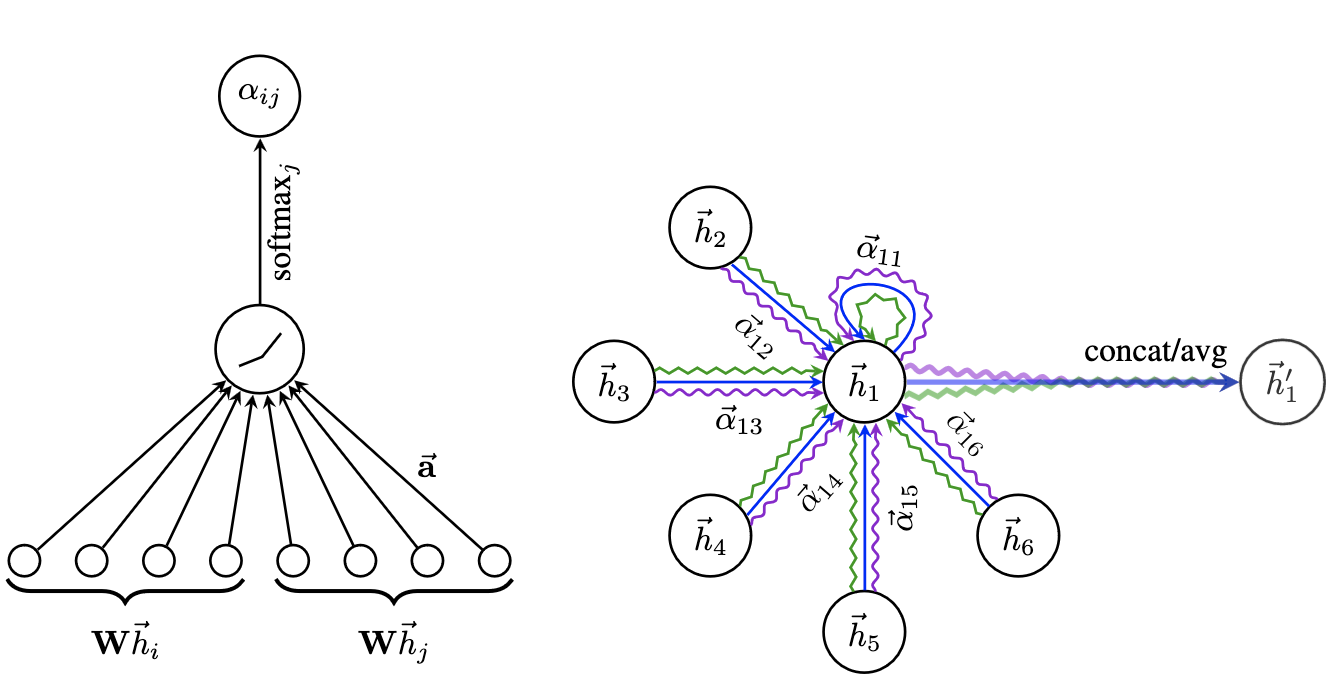
\includegraphics[width=\textwidth]{imgs/gat.png}
    \caption{On the left is the overview of the computation of the attention weights. For each adjacent node an attention weight is computed based on the similarity of their embeddings. On the right there is a visualisation about multi-head attention, which consists of concatenating the result of several attention mechanisms. The figures are taken from the original article \cite{graphatt}.}
    \label{fig:gat}
\end{figure}

More formally, the computation can be described as follows

\begin{equation}
    \bh_j^{(l+1)} = \sigma \left(\sum_{k \in \mathcal{N}_j} \alpha_{jk} \bW^{(l)}\bh_k^{(l)}\right)
\end{equation}

\noindent where $\bW^{l}\in \R^{d\times d}$ are the layer weights and $\alpha_{jk} \in \R$ are the attention weights which are defined by the following formula

\begin{equation}
    \alpha_{jk} = \frac{\exp(\text{LeakyReLU}(\ba \cdot [\bW \bh_j||\bW \bh_k]))}{\sum_{r\in \mathcal{N}_j} \exp(\text{LeakyReLU}(\ba \cdot [\bW \bh_j||\bW \bh_r]))}
\end{equation}

\noindent being $\ba \in \R^{2d'}, \bW \in \R^{d'\times d}$ two learnable projection matrices, LeakyReLU is the leaky rectified linear unit \cite{leakyrelu} and $||$ the concatenation operation. Inspired by the multi-head attention mechanism proposed in \cite{transformer}, the previous attention mechanism can be extended to $H$ heads

\begin{equation}
    \bh_j^{(l+1)} = \bigparallel_{h=1}^H \sigma \left(\sum_{k \in \mathcal{N}_j} \alpha_{jkh} \bW^{(l)}_h\bh_k^{(l)}\right)
\end{equation}

\noindent where now $\bW^{(l)}_h \in \R^{d \times Hd}$, the attention weights are different for each head and sum up to one in each head $\sum_{k\in\mathcal{N}_j}\alpha_{jkh}=1,\ \forall h$ and in the final layer heads are averaged instead of concatenated as explained in \cite{graphatt}.